

\chapter{Introduction}


This chapter introduces the reader to the concept of computational sensing and provides the motivation for the need to address the practical issues in experimental computational sensing. 

Computational sensing is the concept that a joint design of the sensor hardware, often though coding of the analog signal combined with task-specific algorithms can exceed the performance of a traditional sensor, which we call \emph{isomorphic sensors}. While isomorphic sensors can provide flexible sensing in multiple applications. A computational sensor's task specific design---which considers both the architecture of the sensor and coding of the analog signal ---naturally lends to performance increases \cite{neifeld2006taskSpecificSensing}. 

Throughout this chapter and the rest of this dissertation we will provide many examples that highlight the differences between computational and isomorphic sensing. 

Rather than a rigorous discussion, this chapter will discuss some of the major developments and contributions to the field of computational sensing on an intuitive level. This will familiarize the reader with important terminology and techniques common in the computational sensing community. The projects presented in this dissertation are a natural evolution of these developments. A rigorous discussion of the concepts is given in \autoref{chap:Formalism}. Then I will briefly discuss some of the challenges I and many other experimentalists and engineers have faced when developing computational sensing prototypes. Then the chapter will close with a brief look ahead to the rest of the dissertation. 

%History%%%%%%%%%%%%%%%%%%%%

\section{A Historical Development of Computational Sensing}

\subsection{Isomorphic Sensing}

In Greek, the word isomorphic loosely translates to equal in form. Traditional sensors perform isomorphic sensing. In the context of this dissertation, an isomorphic sensor is any sensor which attempts to produce an output signal that resembles the signal-of-interest. In this paradigm, the analog instrument, sampling scheme, and task-specific algorithms are seperated, see Figure \ref{fig:isomorphicsesingflowchart}.


\begin{figure}
    \centering
    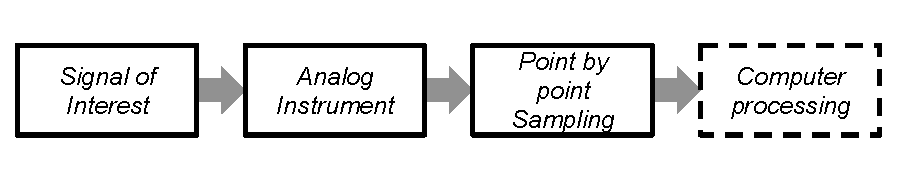
\includegraphics[scale=1]{isomorphicsensorflowchart}
    \caption{A high level view of a traditional sensing scheme. The signal-of-interest is incident upon the analog instrument. The analog instrument forms an isomorphism of the signal which is tern periodically sampled point by point through an analog-to-digital converter (ADC) device. Once the signal is in digital form, post-processing algorithms are often used to perform various tasks such as noise reduction, detection, and classification. Notice that the analog instrument, sampling scheme, and processing are all seperated. }
    \label{fig:isomorphicsesingflowchart}
\end{figure}

A good example of an isomorphic sensor is the photographic camera. In the camera, the signal-of-interest is the object that is being photographed. The analog instrument consists of the lens which is designed and fabricated to produce an intensity distribution---an image---that is nearly diffraction limited at the \gls{fpa}. The \gls{fpa} then samples and quantizes the image and produces a digital representation of the object. Often stored digital image is post-processed using software to increased desired effects such noise removal or to locate the object. 

There are two major components in the camera which determine how well it be used to perform a specific task: the optics and the FPA. Ideally, the optics (the analog instrument in this case) will produce a \gls{psf} which is infinitely small in diameter. For example, in a task such as the detection of a star from several neighboring stars in the night sky, if the  \gls{psf} much larger than the center to center seperation of the two stars in the optical image, it will be quite difficult to detect. A careful reader will note that this is essentially the argument used by Lord Raleigh in proposing his resolution criterion. 

Similarly, the camera must be able to sample the intensity distribution with a small enough resolution---pixel spacing---to be able to produce a digital signal that

As establish by the Raleigh-Criterion [CITE FOURIER OPTICS]the resolution of the optics is limited by diffration. Notice that in the resolution of the camera i

\section{Dissertation Overview}

%This section explores a brief history of the development of nuclear weapons---from their development and first use in 1945 to the buildup of the arms race (\cref{sec:chIntrosecHistorysubsecBuildup}). This culminated in the Cuban Missile Crisis (\cref{sec:chIntrosecHistorysubsecCMC}), which is considered the height of the Cold War. A summary is presented of important treaties signed between the United States (U.S.), Soviet Union (U.S.S.R.) and other nuclear and non-nuclear states over the past several decades in~\cref{sec:chIntrosecHistorysubsecNPT}. To verify compliance with future treaties, new technologies will be needed. The challenges associated with these different problems are summarized in~\cref{sec:chIntrosecHistorysubsecFuture}. More details, and summaries of interesting historical events, can be found in Charles Loeber's book~\citep{IntroBuildingtheBomb}. 




%\bibliographystyle{IEEEtranS}  
%\bibliography{ThesisBib}

